\subsection{Developing surrogates} 

Surrogates are developed using artificial neural networks (ANNs). ANNs are inspired in the human brain. A given network is a combination of different so-called neurons which have certain initial weight and activation functions. These neurons are grouped in different layers. The first layer is called input layer, and the last layer is called the output layer. Other layers between input and output layers are called hidden layers. We use two structures of ANNs.  One structure is developed to estimate PGV, and the other structure is developed to estimate PGV, PGA, SA, and Venv for two horizontal components. Alternative metrics increase signal uniqueness. There is less chance that two signals which are generated with two sets of different input parameters (i.e., $C$,$\alpha$, and $\beta$) have the same PGV, PGA, Venv and SA. Consequently, the optimization algorithm can effectively find the best set of solutions. Fig.~\ref{fig:Figure_ann_structure} shows the structures of networks. The number of neurons in each hidden layer is presented at the top of each layer.

 \begin{figure}
    \centering
    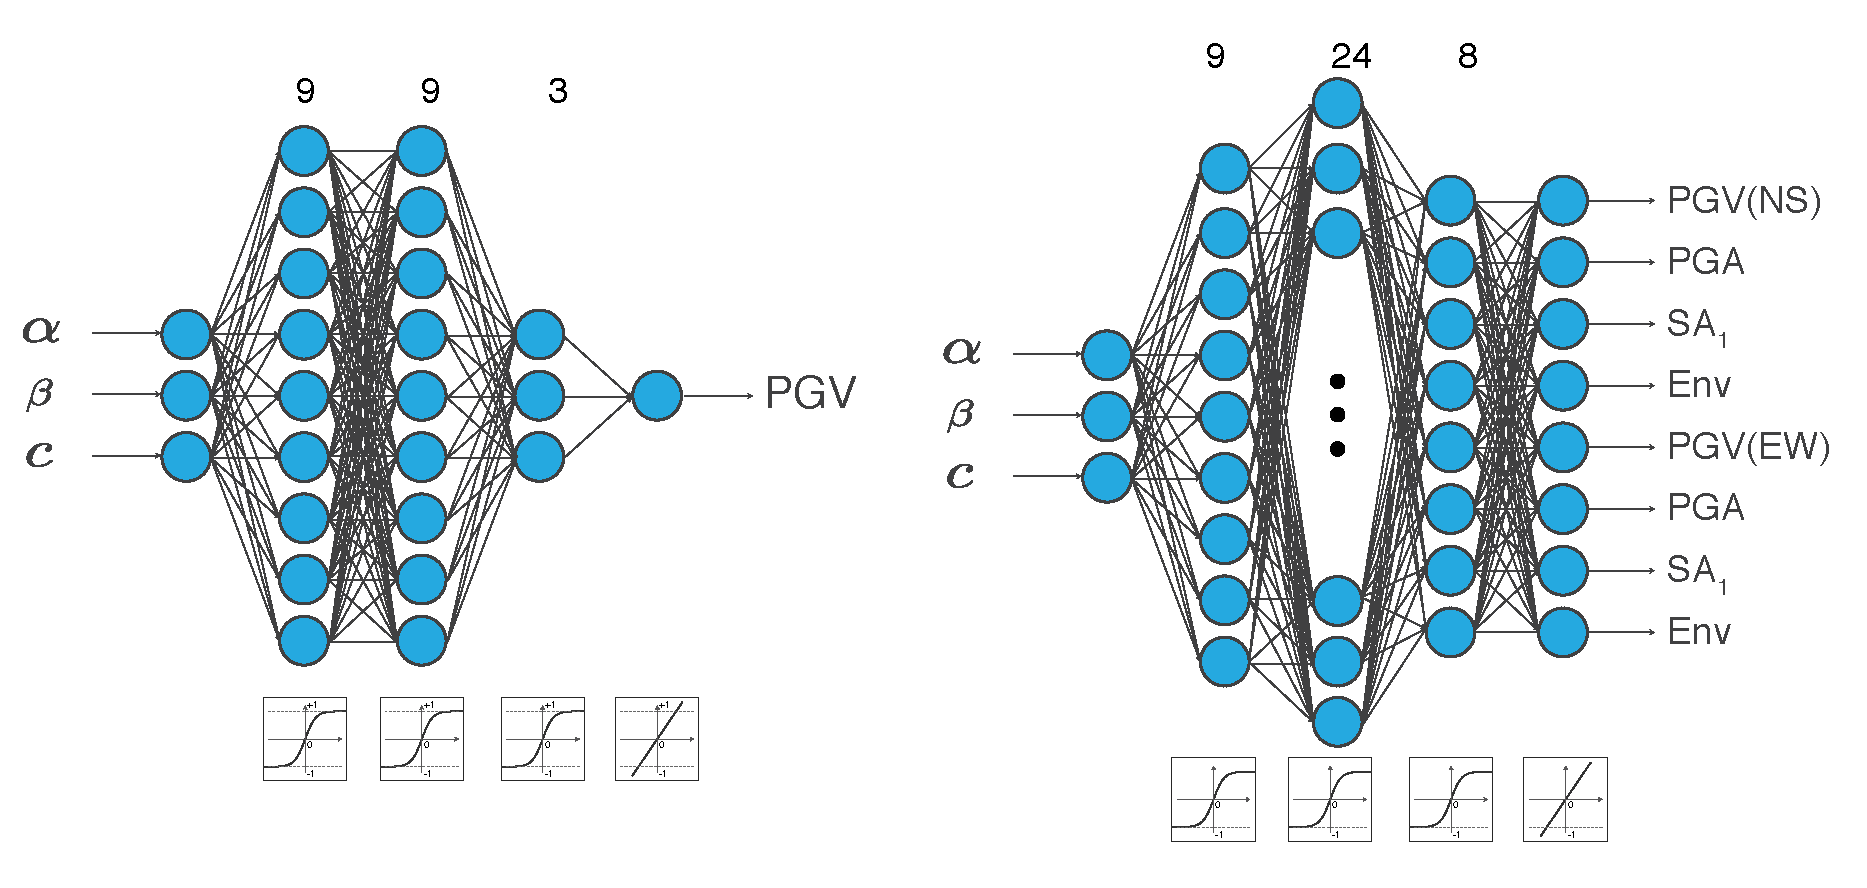
\includegraphics[width=1\textwidth]{figures/pdf/Figure_03.pdf}
    \caption{Feedforward multilayer perceptron neural networks used in the study. Hidden layers use tangent sigmoid and output layer uses linear activation functions. Dots used to simplify the structure for presenting purposes.}
    \label{fig:Figure_ann_structure}
\end{figure}

Input values for all ANNs in this study is \qsvs{} relationship parameters (i.e., $C$, $\alpha$, and $\beta$). All nodes are interconnected, and each layer has an activation function. One can train a network using available data by means of a process during which the weights and bias values associated with the network's neurons are updated so that these will produce output results with increasingly lower residuals in comparison with the input observations. Training ANNs provides a mean to avoid repeated expensive computations. Studying neural network structure and different networks and algorithms are beyond the scope of this study.  In this study, we use feedforward neural networks and Levenberg-Marquardt optimization as a network training function to update weight and bias values. We use linear transfer functions for the last layers and hyperbolic tangent-sigmoid transfer functions for the rest of them. The package is implemented in Matlab programming tool. The algorithm divides the data into three sets including training, validation, and testing dataset. Validation dataset is used to stop training process to avoid overfitting during the training process. An ANN can accurately learn any dataset, provided there is no noise in the data. However, a well trained ANN for one dataset may not be a good predictor for another dataset. This situation is called overfitting. Validation dataset is used to stop the training processing when overfitting occurs. The test dataset is used after fully training data to analyze the functionality of the network. For training ANNs, first, we leave out 5\% of the dataset for the final testing. These data have never been provided to ANNs during the training sessions. We assign 85 and 15\% of remaining data into training and validation datasets.  Neural networks' training process, depending on the size of the networks, is involved with hundreds of thousands of matrix multiplication. Therefore, normalized input values ensure the stability of the networks and improve its internal optimization process in case of inequivalent attributes. We linearly scale the data into $[-1,1]$ using

\begin{equation}
X_{norm} = \frac{2*(X-X_{min})}{(X_{max}-X_{min})}-1
\end{equation}

where $X_{norm}$ is the normalized value; $X_{min}$ and $X_{max}$ are minimum and maximum value of $X$ vector, respectively. The performance is computed by use of mean squared error (RMSE) between the network predicted values and observation. As of epoch number increases, the network learns to predict the data with high accuracy. An epoch is one complete presentation of the dataset to be learned to an ANN. For a small dataset where all data can fit into the system at once, one epoch is one iteration. In general, with increasing training data, the network functionality increases for unseen data and becomes more generalizable. Generalizability means that the trained ANN can accurately estimate the output values from input values that it has never seen them before. In many cases, developing training data can cost a considerable amount of computational and financial resources. Studying the methods for generating the most appropriate training data is beyond the scope of this paper. In this study, we generate enough training data and study the effect of training data size in network performance. We use bootstrap aggregating (bagging) predictors to increase the generalizability and accuracy of predictors \citep{Breiman_1996_ML}. Bagging is a method for generating multiple versions of a predictor and using these to get an aggregated predictor. We use the trained networks in optimization process as surrogates in the cost functions. 


